\documentclass[main.tex]{subfiles}
\begin{document}
\chapter{Discussion}
\section{Summary of Findings}
\subsection{Robotic Arm Offset}
The simulation was able to show convergence of the VHCs for a large range of initial conditions. Figure \ref{fig:graph-robotarm} shows a few sample plots. Note that the VHC was adjusted to account for the behaviour of angles as $\ree/2\pi$.

One plot, in the top left, appears as not converging: this corresponds to an initial where $\theta=\phi$. In fact, this is just a floating point error and the divergence is on the order of $10^-13$. While not a critical issue, it is recommended that future iterations of the code account for these arithmetic inconsistencies.
\begin{figure}[h]
    \centering
    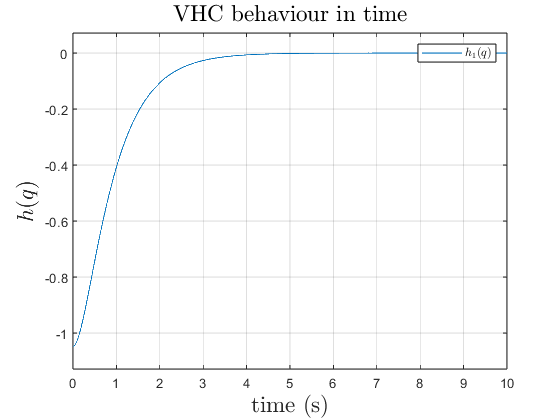
\includegraphics[width=0.48\textwidth]{assets/rao1.png}
    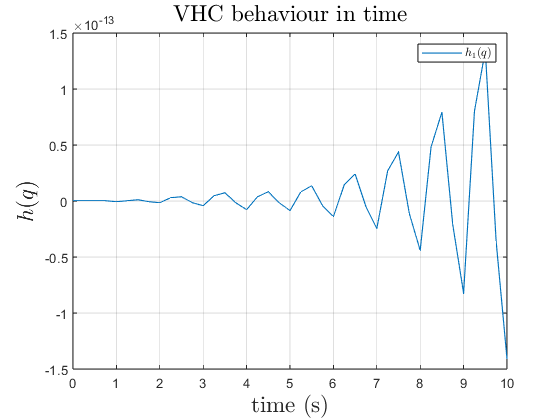
\includegraphics[width=0.48\textwidth]{assets/rao2.png}
    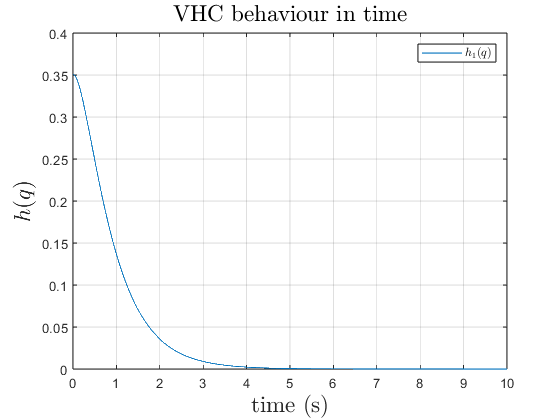
\includegraphics[width=0.48\textwidth]{assets/rao3.png}
    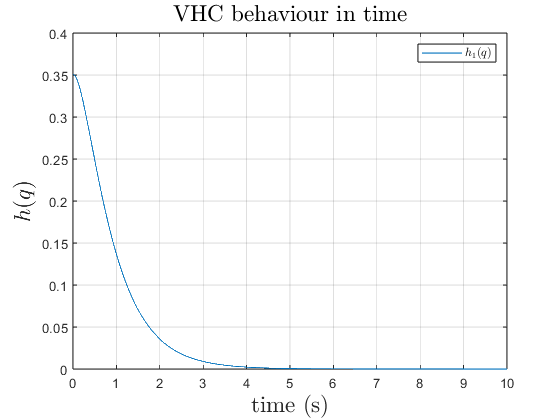
\includegraphics[width=0.48\textwidth]{assets/rao4.png}
    \caption{Plot showing convergence of the VHCs (control error) towards zero on the Offset Robotic Arm model. Here, the constraint is defined using the equivalent $h:=\arg\cbr{\exp(i[\theta-\phi])}$.}
    \label{fig:graph-robotarm}
\end{figure}

\subsection{Spherical Pendulum}
Figure \ref{fig:graph-pendulum} shows convergence for the spherical pendulum subject to a range of initial conditions. The top left plot appears to converge slowly, and times out before the VHC gets close to zero. In this case, it is recommended to review the control constants $K_P,K_D$ to allow for faster convergence. The LQR function in Matlab can also be used to achieve optimal control.
\begin{figure}[h]
    \centering
    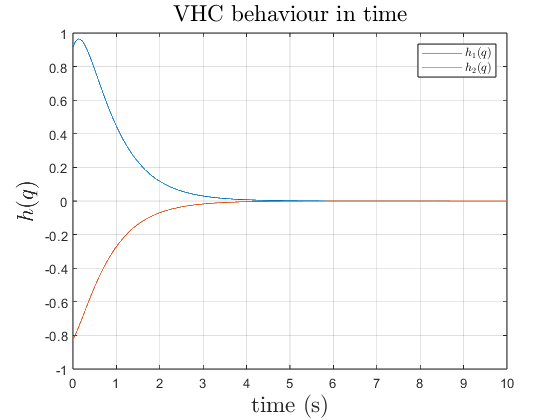
\includegraphics[width=0.48\textwidth]{assets/sp1.png}
    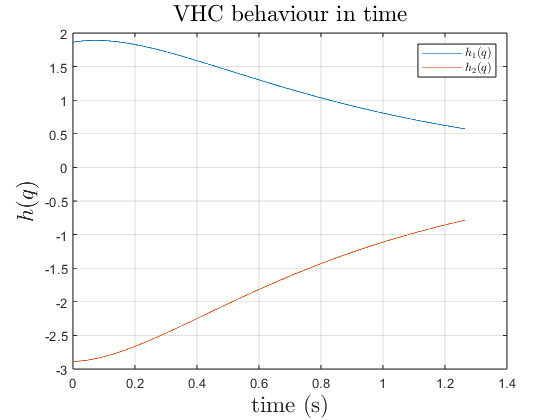
\includegraphics[width=0.48\textwidth]{assets/sp2.png}
    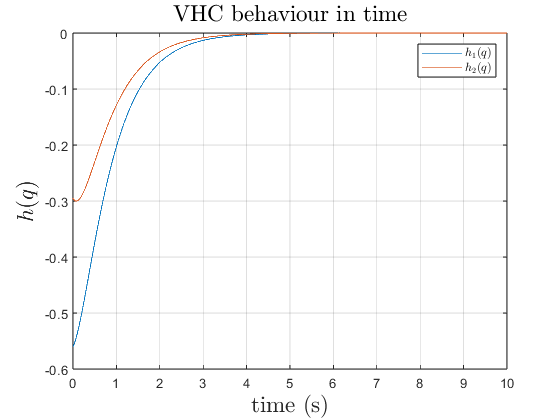
\includegraphics[width=0.48\textwidth]{assets/sp3.png}
    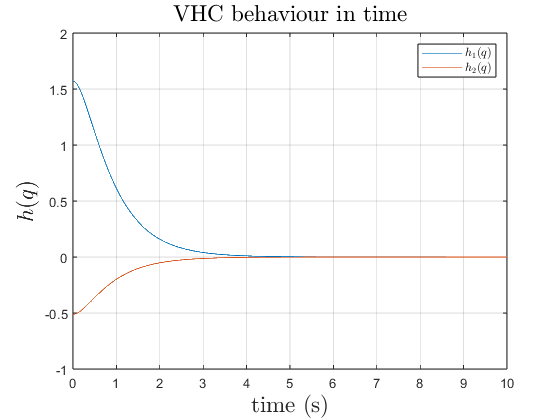
\includegraphics[width=0.48\textwidth]{assets/sp4.png}
        \caption{Plot showing convergence of the VHCs (control error) towards zero on the Spherical Pendulum model. Here, the constraint is defined $h_1:=\theta-\phi, h_2=\psi-\frac{\pi}{4}\tanh \rho.$}
    \label{fig:graph-pendulum}
\end{figure}

\section{Future Research}
\subsection{Analyze further examples}
From Section \ref{sec:robotarmoffset}, the Robotic Arm Offset example is somewhat trivial, as its reduced form is apparent at all points on the constraint manifold $\mathcal{C}$.

Therefore, future research should explore further examples of mechanical systems, with the aim to provide a more concrete illustration of the technique of dynamical reduction described by McCarthy et al\cite{mccarthy}. 
Tedrake's notes on Underactuated Robotics\cite{underactuated} contain some examples that (with perhaps some modifications) could be used in a continuation of this work. It is recommended to choose systems with 4 degrees of freedom and 2 actuators--systems with 3 degrees of freedom and 1 actuator may not be as interesting to study.

\subsection{Metrizability of the connection}
If the connection on the constraint manifold is metrizable, the dynamics of the VHC-constrained system are Euler-Lagrange\cite{mccarthy}. It would be of interest to determine whether this applies to both systems. Euler-Lagrange systems are well-studied, and if the dynamics are indeed so, the system would be easy to model using the tried and tested strategies.
\end{document}